\subsection{Augmentation du nombre d'épisodes}

\subsubsection{Configuration, modifications et résultats attendus}

Nous décidons d'augmenter le nombre d'épisodes qui servent à entrainer notre
algorithme. Comme le montre les courbes de la perte de la politique des
figures~\ref{fig:sac:results2} et~\ref{fig:sac:results3}, à partir de \(300\)
épisodes, la fonction est décroissante. Nous décidons d'augmenter le nombre
d'épisodes (\(1500\) épisodes) pour voir si la fonction perte de la politique
converge vers \(0\) comme nous pouvons l'espérer.

Nous avons vu en fixant le paramètre \(\alpha\), une convergence qui semble être
plus rapide. Nous allons le vérifier en faisant une exécution pour \(\alpha\)
constant et pour \(\alpha\) appris sur \(1500\) épisodes répétés \(10\) fois. Nous pensons
qu'avec ce paramètre fixé, la convergence sera un peu plus rapide.

\subsubsection{Résultats et analyse}

\begin{figure}[H]
    \centering
    \begin{subfigure}{0.45\textwidth}
        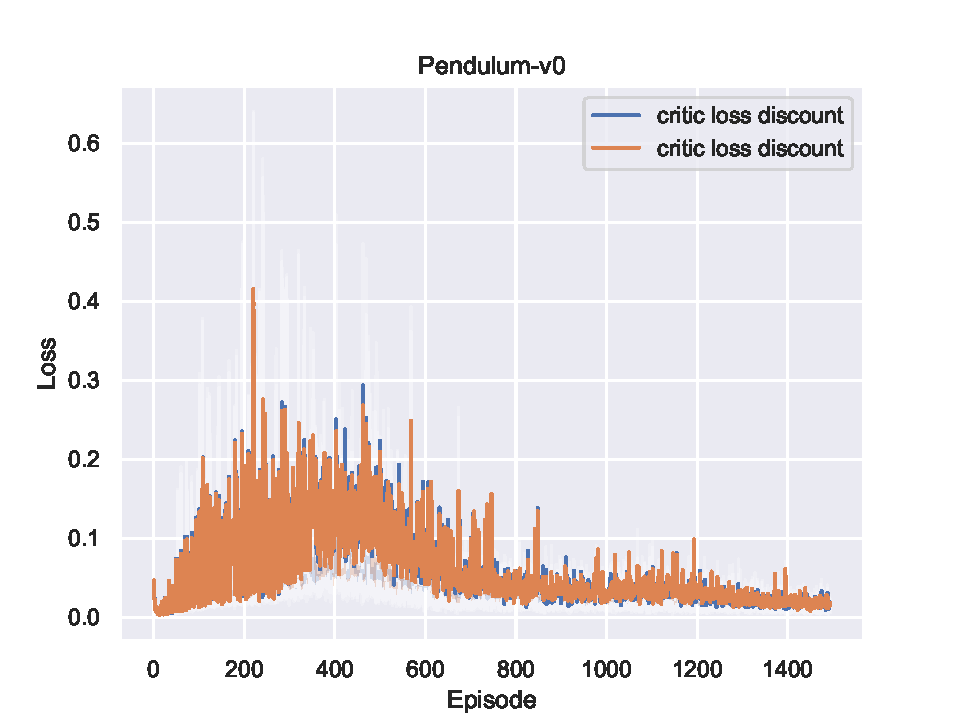
\includegraphics[width=\textwidth]{figures/sac_itr4/a_fixed/critic_loss_Pendulum-v0_pg_dataset_td_trajs_1500_update_threshold_1000_nb_updates_20_gamma_0.98_tau_0.01_nstep_5_lr_act_0.0005_lr_critic_0.001_init_alpha_0.02_lr_alpha_0.0_target_entropy_alpha_-1.0pg.pdf}
        \caption{Fonction de perte de la critique avec \(\alpha\) fixé}
    \end{subfigure}
    \begin{subfigure}{0.45\textwidth}
        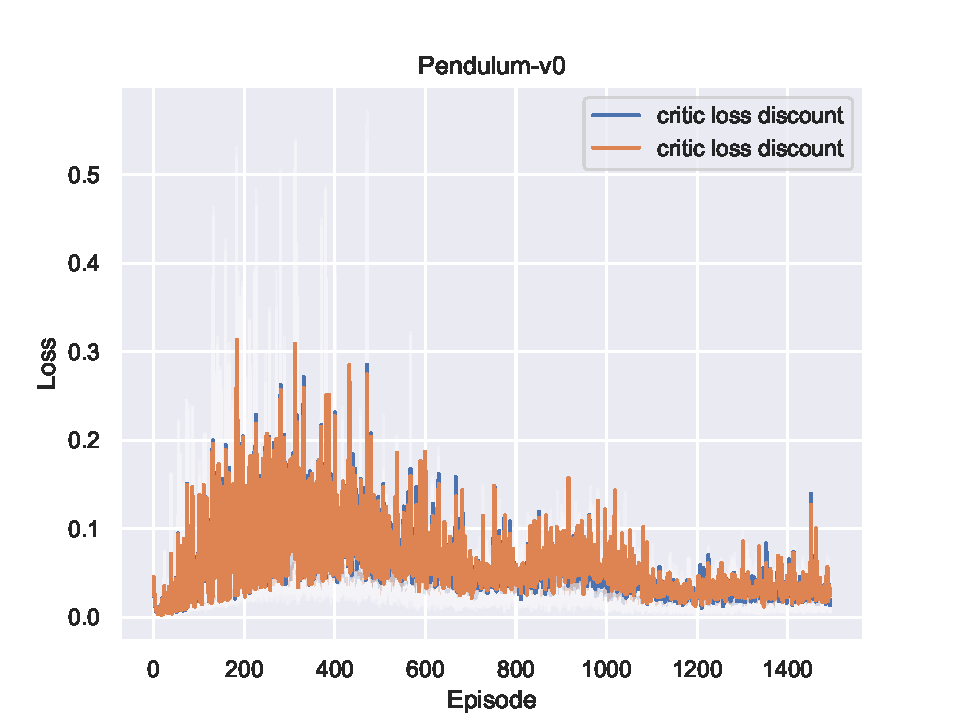
\includegraphics[width=\textwidth]{figures/sac_itr4/a_learned/critic_loss_Pendulum-v0_pg_dataset_td_trajs_1500_update_threshold_1000_nb_updates_20_gamma_0.98_tau_0.01_nstep_5_lr_act_0.0005_lr_critic_0.001_init_alpha_0.02_lr_alpha_0.001_target_entropy_alpha_-1.0pg.pdf}
        \caption{Fonction de perte de la critique avec \(\alpha\) appris}
    \end{subfigure}
    \caption{Comparaison des fonctions de perte des critiques}\label{fig:sac:critics_loss4}
\end{figure}

Nous observons sur la figure~\ref{fig:sac:critics_loss4} que la tendance générale est commune dans les deux cas. Au début
de l'apprentissage, la perte est très bruitée et croît légèrement avant de
tendre vers zero avec moins de bruit. Cependant lorsque \(\alpha\) est appris,
la phase de décroissance de la perte est plus lente et présente plus
d'irrégularités. Nous pouvons affirmer que la fixation de \(\alpha\) est une
bonne idée.

\begin{figure}[H]
    \centering
    \begin{subfigure}{0.45\textwidth}
        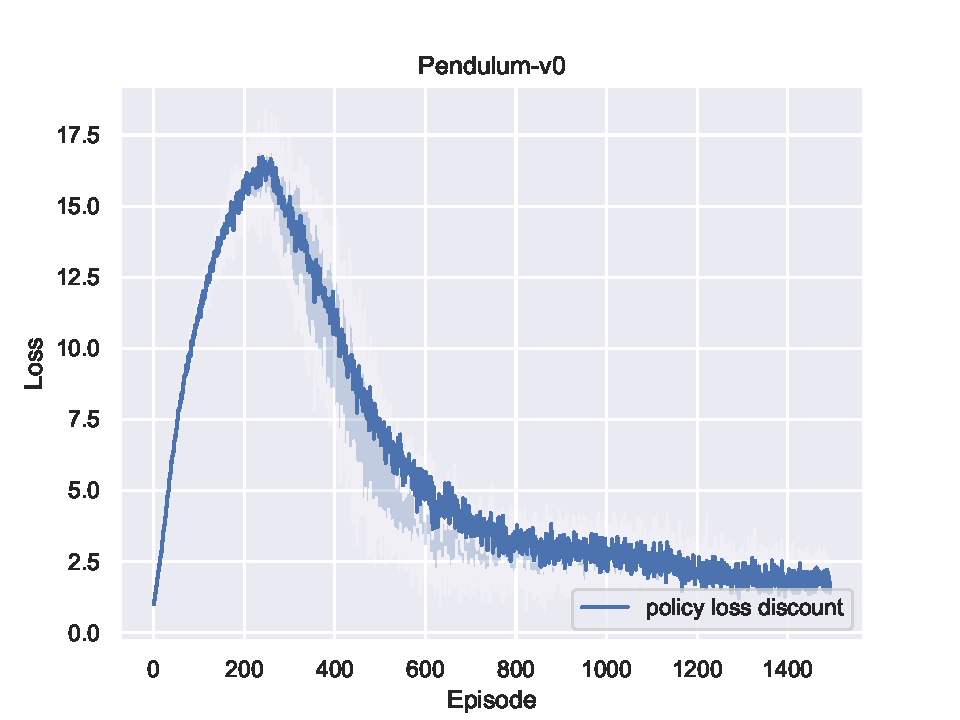
\includegraphics[width=\textwidth]{figures/sac_itr4/a_fixed/policy_loss_Pendulum-v0_pg_dataset_td_trajs_1500_update_threshold_1000_nb_updates_20_gamma_0.98_tau_0.01_nstep_5_lr_act_0.0005_lr_critic_0.001_init_alpha_0.02_lr_alpha_0.0_target_entropy_alpha_-1.0pg.pdf}
        \caption{Fonction de perte de la politique avec \(\alpha\) fixé}
    \end{subfigure}
    \begin{subfigure}{0.45\textwidth}
        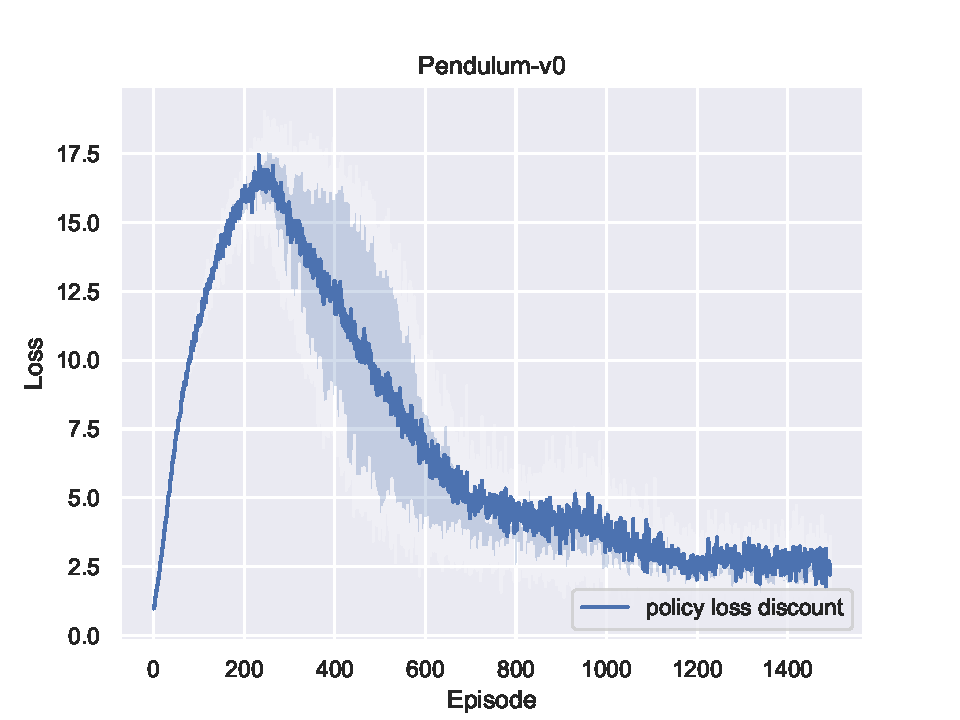
\includegraphics[width=\textwidth]{figures/sac_itr4/a_learned/policy_loss_Pendulum-v0_pg_dataset_td_trajs_1500_update_threshold_1000_nb_updates_20_gamma_0.98_tau_0.01_nstep_5_lr_act_0.0005_lr_critic_0.001_init_alpha_0.02_lr_alpha_0.001_target_entropy_alpha_-1.0pg.pdf}
        \caption{Fonction de perte de la politique avec \(\alpha\) appris}
    \end{subfigure}
    \caption{Comparaison des fonctions de perte des politique}\label{fig:sac:policy_loss4}
\end{figure}

L'évolution globale de la fonction de perte de la politique sur la figure~\ref{fig:sac:policy_loss4} est également
identique aux deux cas. Nous pouvons cependant constater que la répétabilité de l'expérience est meilleur avec la fixation de \(\alpha\). Cette fixation ajoute aussi une meilleur stabilité dans la décroissance de la fonction perte et baisse légèrement le minimum atteint en fin d'apprentissage. En effet, il passe d'environ \( 2.5\) à environ \( 1.8\) avec la fixation. Finalement, nous observons que la raideur de la pente de la fonction après \(200\) épisodes est plus élevée lorsque \(\alpha\) n'est pas appris. La fonction atteint la valeur \(7.5\) vers le \(500\)e épisode lorsque \(\alpha\) est fixé alors qu'elle atteint la même valeur autour du \(600\)e épisode lorsque \(\alpha\) est appris. Cela conforte notre opinion sur la fixation de ce paramètre.

\begin{figure}[H]
    \centering
    \begin{subfigure}{0.45\textwidth}
        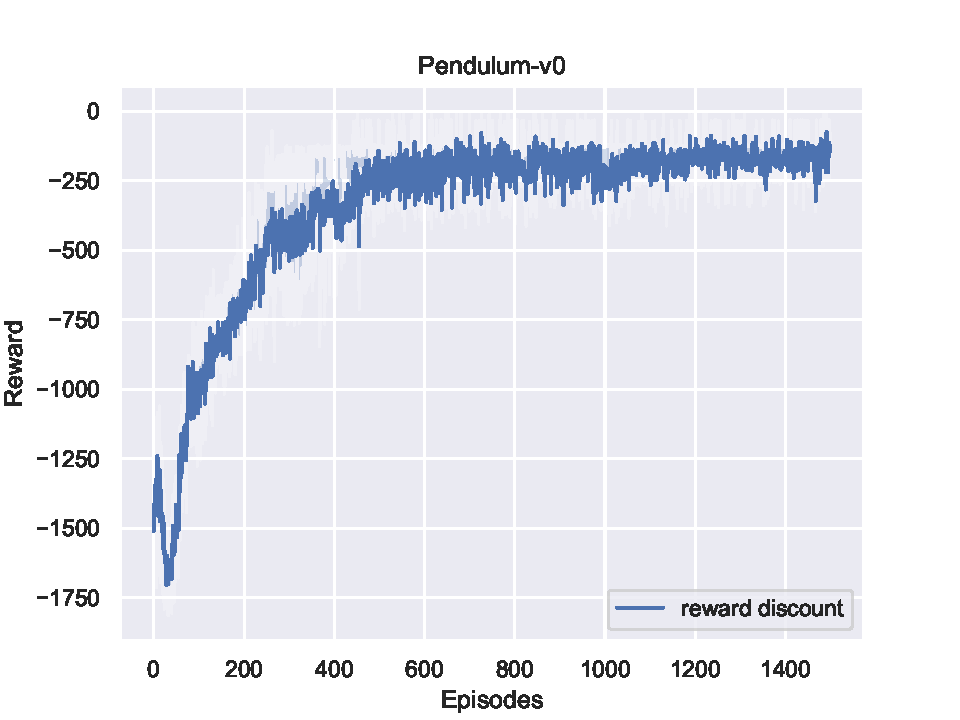
\includegraphics[width=\textwidth]{figures/sac_itr4/a_fixed/rewards_Pendulum-v0_pg_dataset_td_trajs_1500_update_threshold_1000_nb_updates_20_gamma_0.98_tau_0.01_nstep_5_lr_act_0.0005_lr_critic_0.001_init_alpha_0.02_lr_alpha_0.0_target_entropy_alpha_-1.0.pdf}
        \caption{Récompenses obtnues avec \(\alpha\) fixé}
    \end{subfigure}
    \begin{subfigure}{0.45\textwidth}
        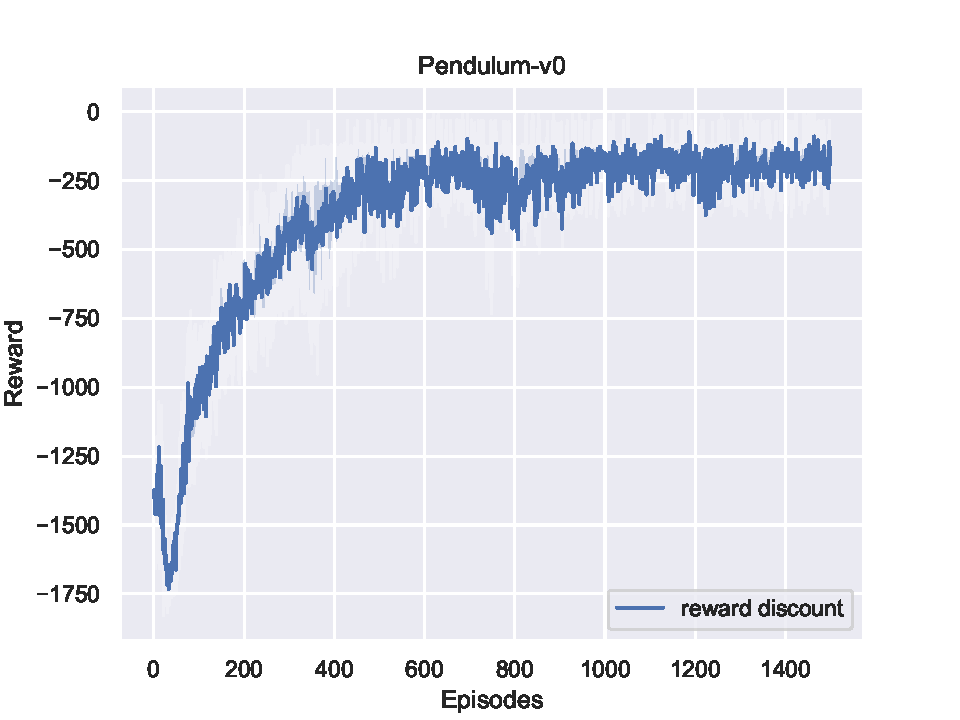
\includegraphics[width=\textwidth]{figures/sac_itr4/a_learned/rewards_Pendulum-v0_pg_dataset_td_trajs_1500_update_threshold_1000_nb_updates_20_gamma_0.98_tau_0.01_nstep_5_lr_act_0.0005_lr_critic_0.001_init_alpha_0.02_lr_alpha_0.001_target_entropy_alpha_-1.0.pdf}
        \caption{Récompenses obtnues avec \(\alpha\) appris}
    \end{subfigure}
    \caption{Comparaison des récompenses obtenues}\label{fig:sac:rewards4}
\end{figure}

Encore une fois, les courbes de la figure~\ref{fig:sac:rewards4} sont similaires et ne présentent que de légères différences. Lorsque le paramètre \(\alpha\) est fixé l'évolution de la récompense est plus stable et confirme définitivement que nous devons garder \(\alpha\) fixe pour avoir une politique optimale et efficace sur de nombreuse trajectoires.

\begin{figure}[H]
    \centering
    \begin{subfigure}{0.45\textwidth}
        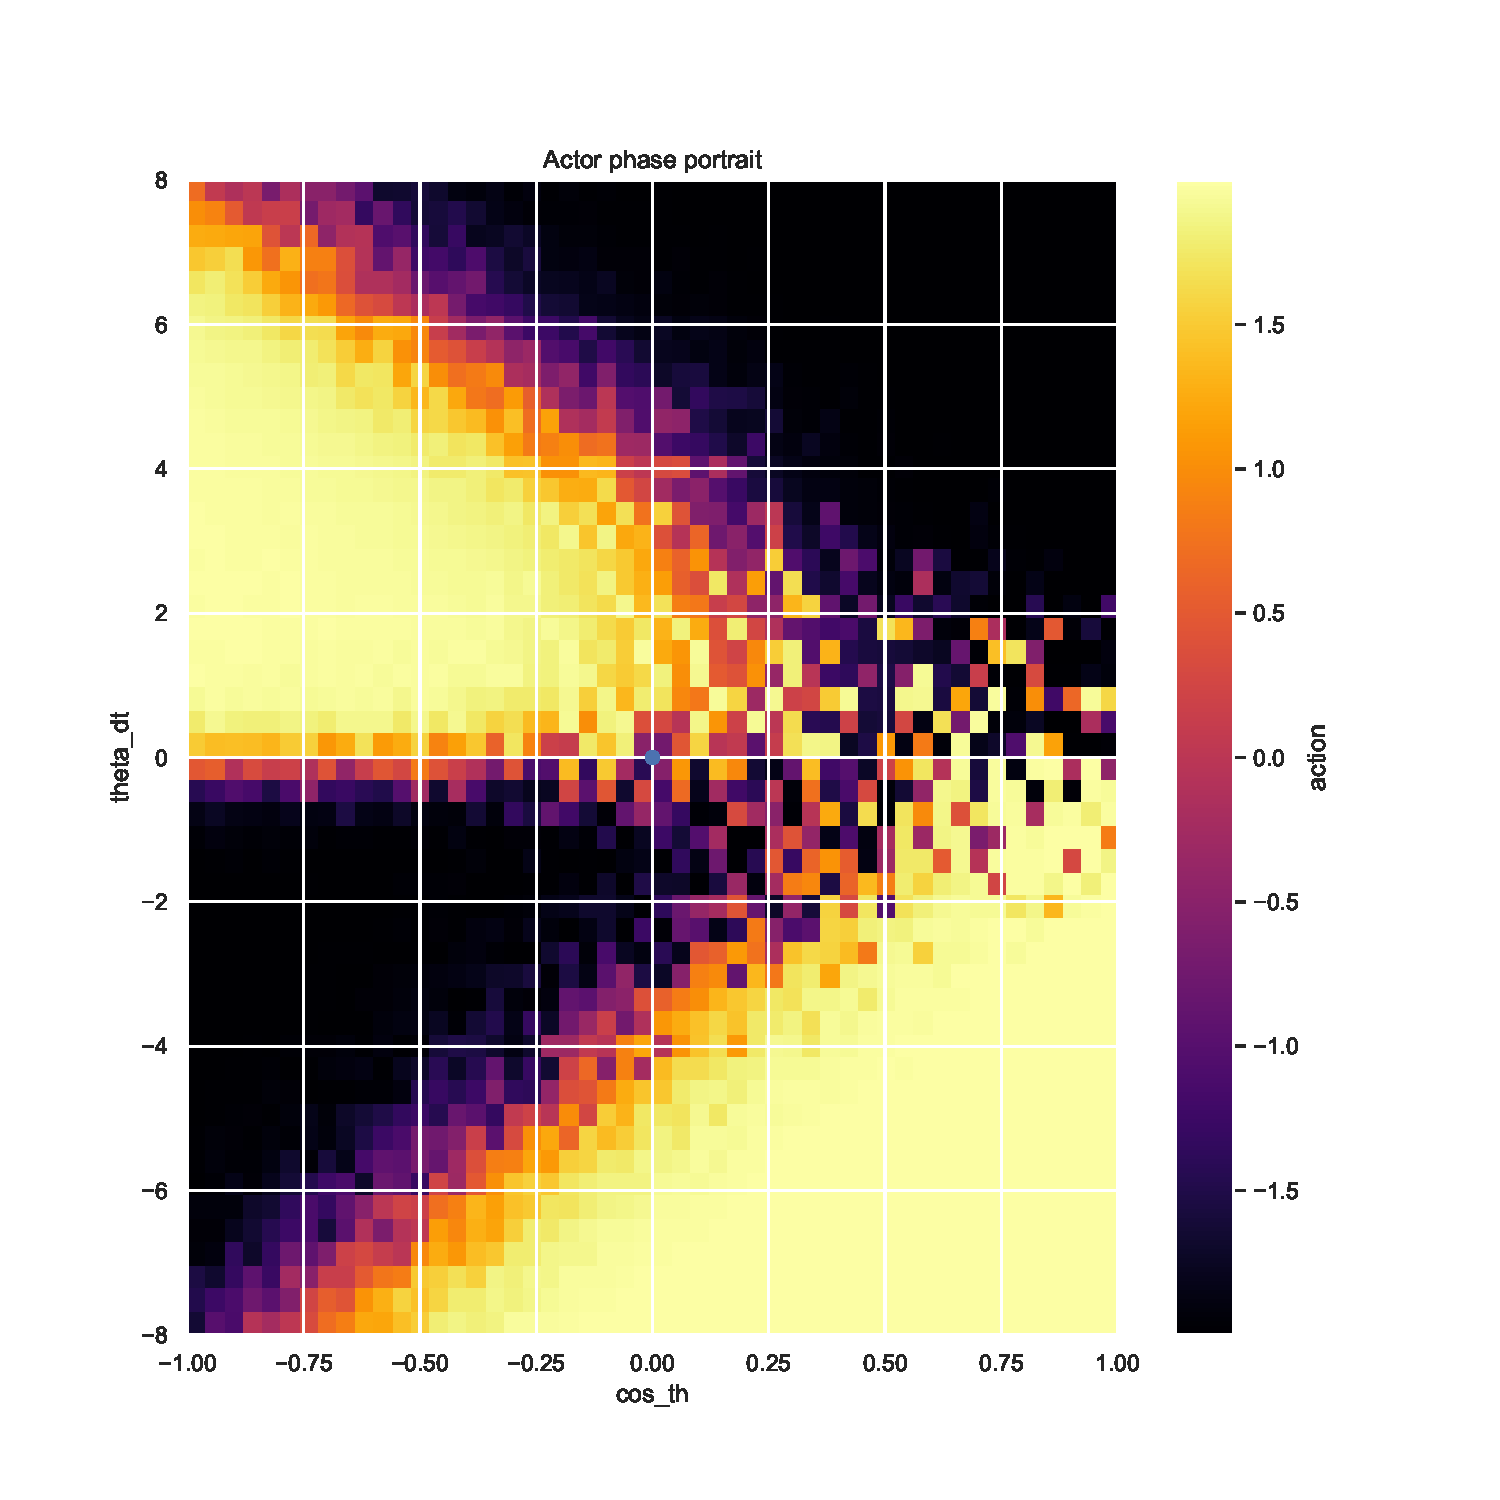
\includegraphics[width=\textwidth]{figures/sac_itr4/a_fixed/5_actor_pg__post_Pendulum-v0.pdf}
        \caption{Valeurs de la politique obtnues avec \(\alpha\) fixé}
    \end{subfigure}
    \begin{subfigure}{0.45\textwidth}
        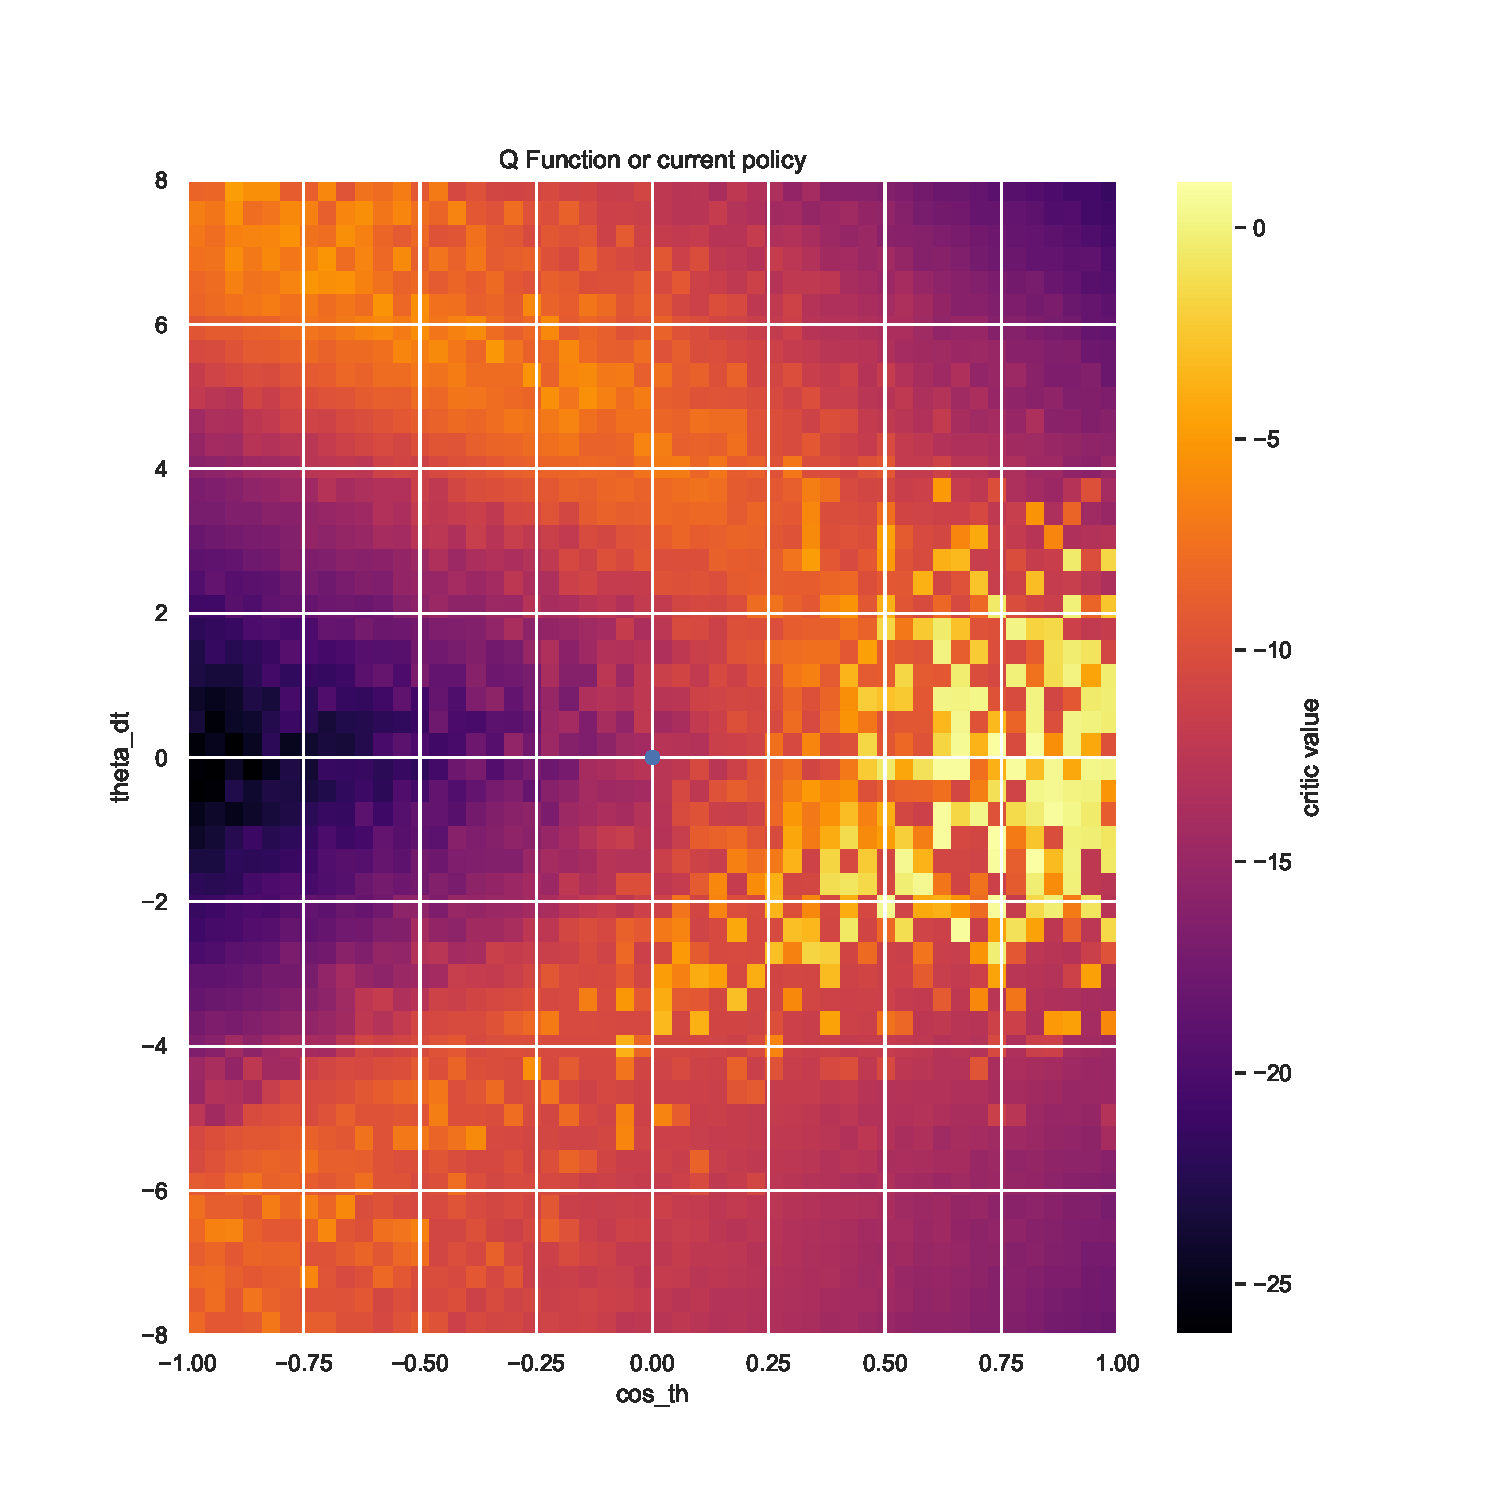
\includegraphics[width=\textwidth]{figures/sac_itr4/a_fixed/5_critic_pg_q2_post_Pendulum-v0.pdf}
        \caption{Valeurs d'une des critiques obtnues avec \(\alpha\) fixé}
    \end{subfigure}
    \caption{Politique et critique obtenues après apprentissage avec \(\alpha\) fixé}\label{fig:sac:heatmap4}
\end{figure}

Nous pouvons voir sur la figure~\ref{fig:sac:heatmap4} que nous avons un chevron > bien prononcé sur la \emph{heatmap} de la critique. Ce chevron permet d'expliquer la transition douce sur la \emph{heatmap} de la politique pour les valeurs négatives de \(\cos(\theta)\), et ce quelque soit le sens de rotation initiale du pendule. Ce résultat n'est pas aussi probant lorsque \(\alpha\) est appris. Il resterai encore à paufiner la zone autour de \(\cos(\theta) = 1\) pour avoir un système le plus efficace paussible.